\documentclass[a4paper]{article}
\linespread{1.6}
\usepackage{geometry}
\usepackage{setspace}
\usepackage{amsmath}
\usepackage{amssymb}
\usepackage{enumerate}
\usepackage{subfigure}
\usepackage{caption}
\usepackage{listings}
\usepackage{float}
\captionsetup{font = footnotesize}
\usepackage[pdftex]{graphicx}
\geometry{left=1cm,right=1cm,top=2.5cm,bottom=2.5cm}

\begin{document}
\begin{spacing}{2.0}
\begin{flushleft}\begin{huge}EEE6561  Fundamentals of Biometric Identification   Homework 4\end{huge}
\end{flushleft}
\begin{flushright}\begin{Large}Hudanyun Sheng\end{Large}\end{flushright}

\section*{\huge\textbf{ Part \uppercase\expandafter{\romannumeral1} Fingerprint Classification / Data Preparation}  }
	\normalsize
		The fingerprints are shown in below:
	
\begin{figure}[h]
	\begin{minipage}[t]{0.24\linewidth}
	\centering
	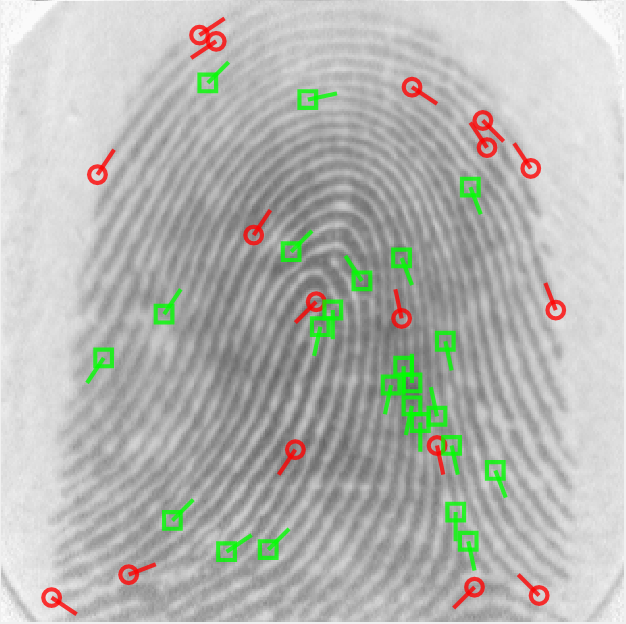
\includegraphics[width = 1.8in]{1.png}
	\caption{Fingerprint1.}
	\label{scoreDis}
	\end{minipage}
	\begin{minipage}[t]{0.24\linewidth}
	\centering
	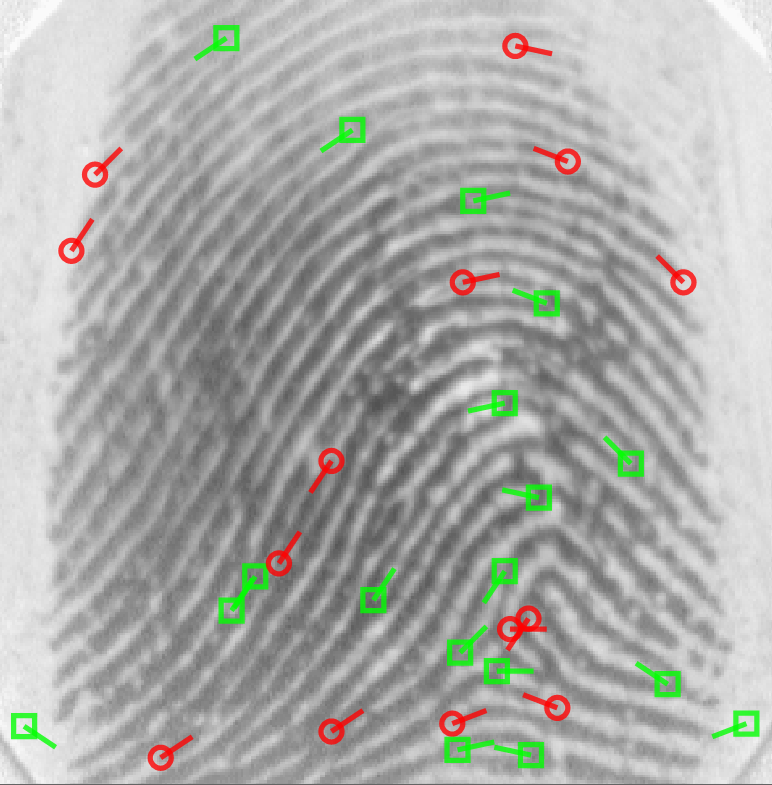
\includegraphics[width = 1.8in]{2.png}
	\caption{Fingerprint2.}
	\label{CMC}
	\end{minipage}
	\begin{minipage}[t]{0.24\linewidth}
	\centering
	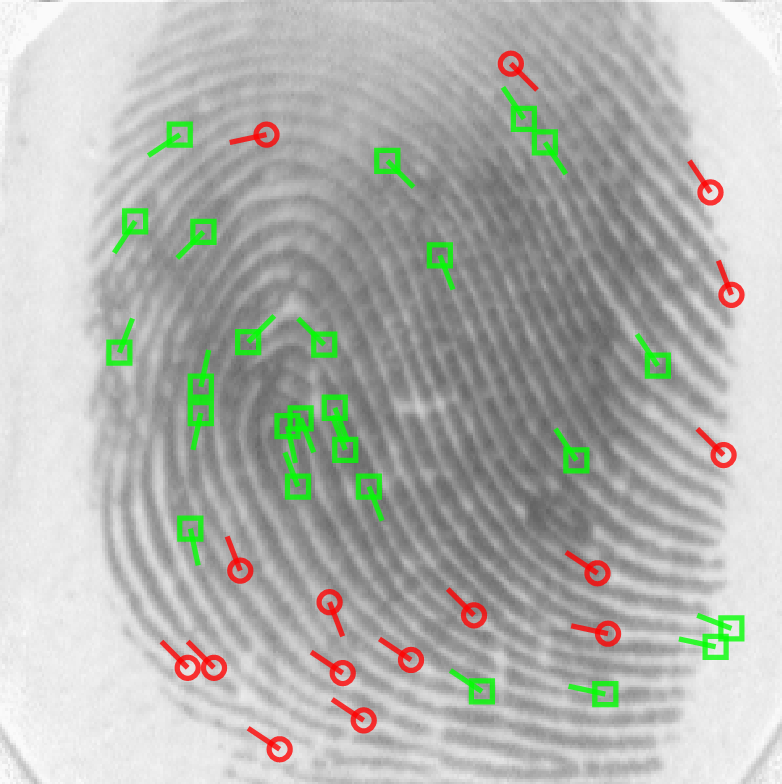
\includegraphics[width = 1.8in]{3.png}
	\caption{Fingerprint3.}
	\label{ROC}
	\end{minipage}
	\begin{minipage}[t]{0.24\linewidth}
	\centering
	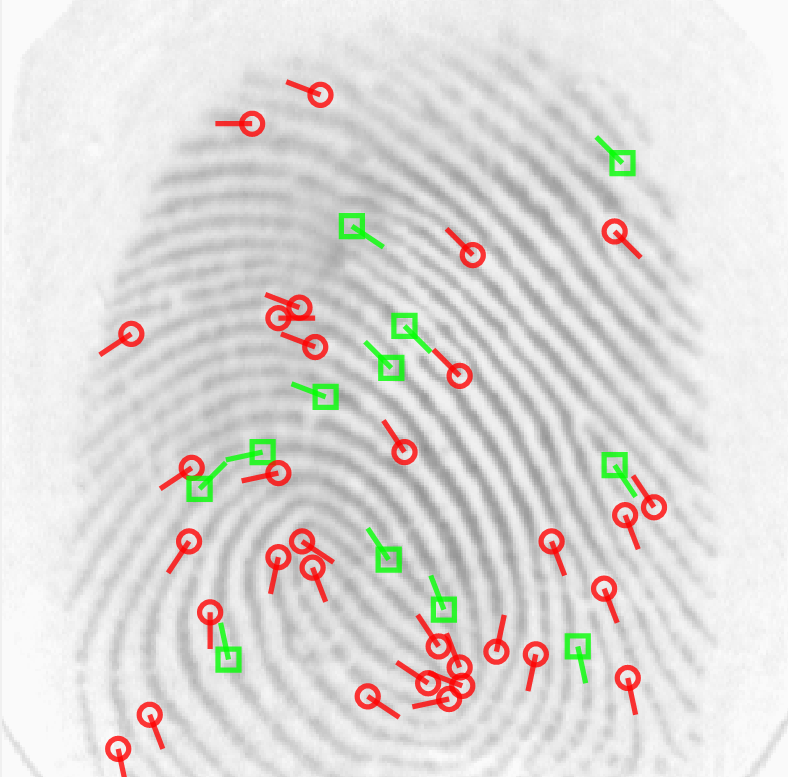
\includegraphics[width = 1.8in]{4.png}
	\caption{Fingerprint4.}
	\label{ROC}
	\end{minipage}
	\end{figure}
\begin{figure}[h]	
	\begin{minipage}[t]{0.3\linewidth}
	\centering
	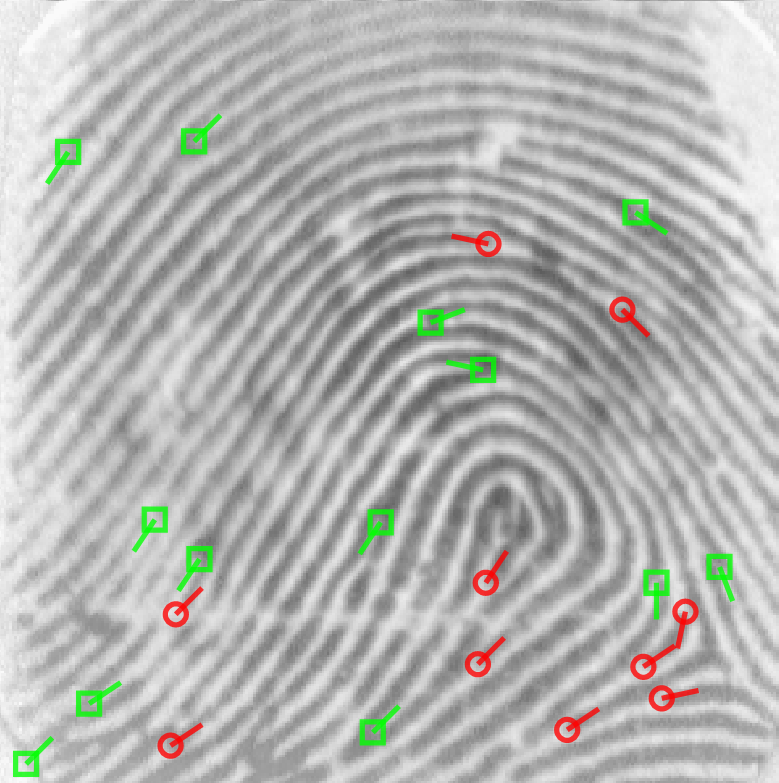
\includegraphics[width = 1.8in]{5.png}
	\caption{Fingerprint5.}
	\label{scoreDis}
	\end{minipage}
	\begin{minipage}[t]{0.3\linewidth}
	\centering
	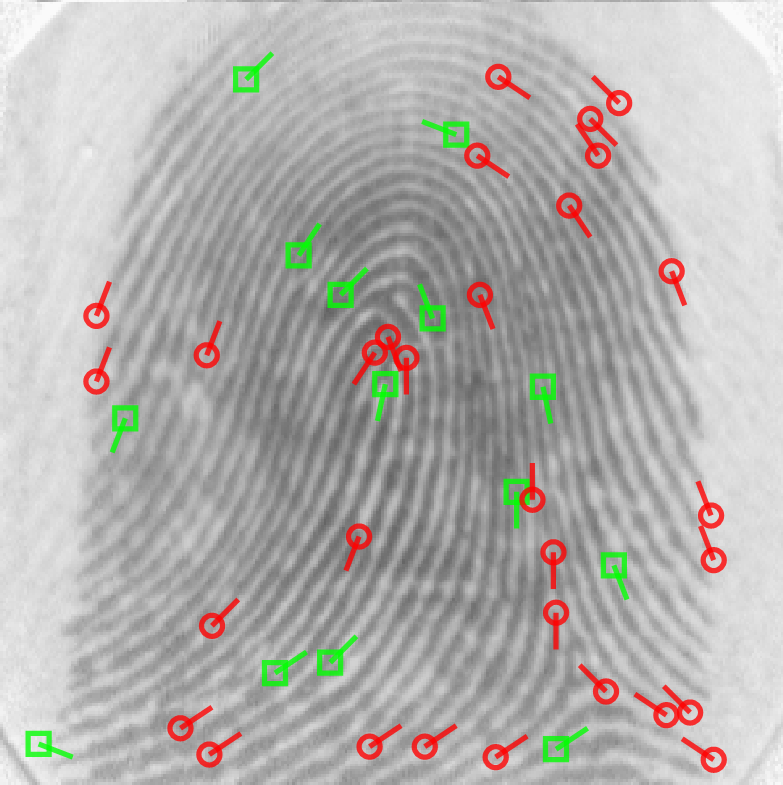
\includegraphics[width = 1.8in]{6.png}
	\caption{Fingerprint6.}
	\label{CMC}
	\end{minipage}
	\begin{minipage}[t]{0.3\linewidth}
	\centering
	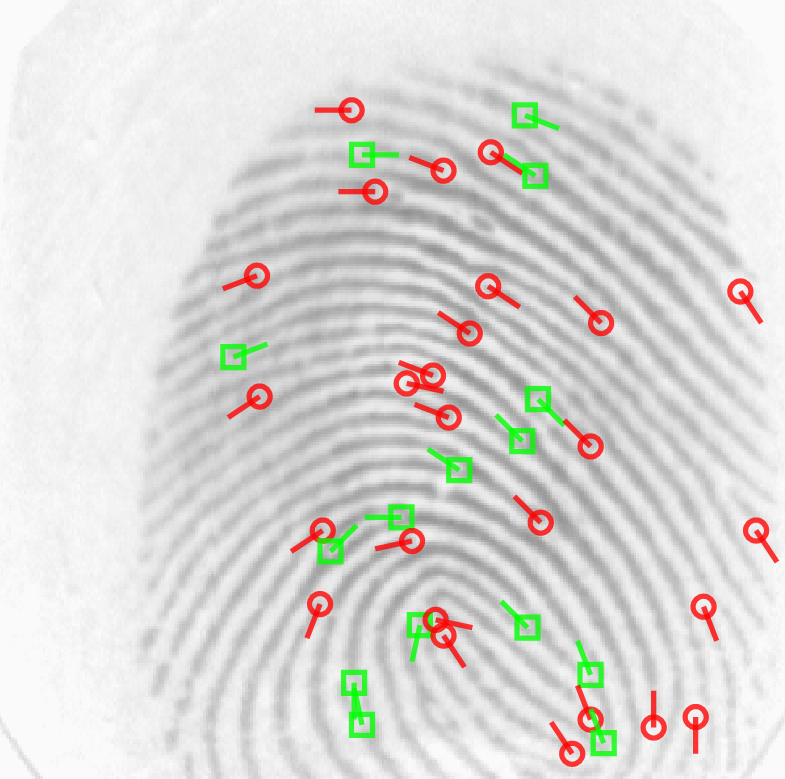
\includegraphics[width = 1.8in]{7.png}
	\caption{Fingerprint7.}
	\end{minipage}
	\end{figure}
	
	\begin{enumerate}[(a)]

	
	\item Using the provided fingerprint viewer software and images, classify the seven fingerprints into the 	six main fingerprint classes discussed in class.\\
	\textbf{1: left loop, 2: left loop, 3: right loop,  4: twin loop, 5: left loop, 6: left loot, 7: twin loop.}
	
	\item The bottom of the fingerprint viewer software window provides information on the minutiae extracted from the fingerprint image. Save the information regarding the minutiae points into seven separate text files consisting of three columns. The first column is the x-value, the second column is the y-value and the third columns is the $\theta$-value. The software expresses the minutiae direction in its own coordinate system that is not degrees. Each quadrant is quantized to eight different values. To obtain the $\theta$-value in degrees, it should be multiplied by 11.25.
	\end{enumerate}
	
\section*{\huge\textbf{ Part \uppercase\expandafter{\romannumeral2} Fingerprint Transformation}  }
	\normalsize
	The values of $\Delta \theta$ are shown as in the degrees.
	\begin{figure}[htbp]
	\centering
	\includegraphics[width = 7.5in]{table1withAngle.png}
	\label{f1}
	\end{figure}
	
\newpage	
\section*{\huge\textbf{ Part \uppercase\expandafter{\romannumeral3} Fingerprint Pairing}  }
	\normalsize
	The resulting table is shown below. The angles are shown in radians.
	
	\begin{figure}[htbp]
	\centering
	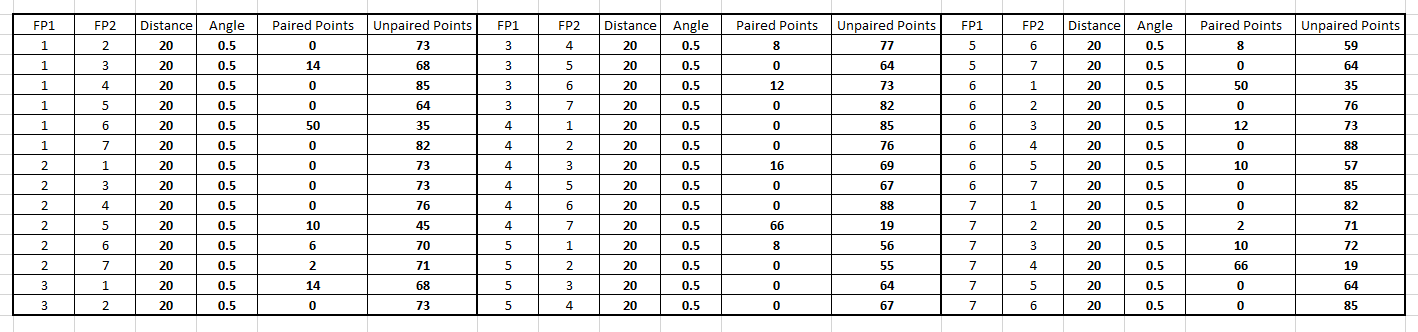
\includegraphics[width = 7.5in]{table2_20.png}
	\label{t}
	\end{figure}
	
	The average number of minutiae points paired is about 8 for each pair of one probe fingerprint with one gallery fingerprint. The thresholds for the distances as well as the angles are chosen to be ones not too large - too large a threshold would cause large false positive rates; nor too small, too small a threshold would cause the paired ratio for every pair look the same. Based on these thoughts, I decided to use the threshold for distance to be 20, the threshold for angle to be 0.5 radians.
	Based on the results, I believe that images 1 and 6 may possibly belong to the same individual, and images 4 and 7 may possibly belong to the same individual. Which result from the fact that this pair of fingerprints own stable high ratio of pair, even when I set a rather small threshold.
	
	 
	
  

	
	
	%\newpage
	%\large{Attached are code for part \uppercase\expandafter{\romannumeral1} :}
	%\normalsize
	%\begin{lstlisting}
	
	%\end{lstlisting}
	
	%\newpage
	%\large{Attached are code for part \uppercase\expandafter{\romannumeral2} }:
	%\normalsize
	%\begin{lstlisting}
	
	%\end{lstlisting}

	
\end{spacing}
\end{document}